\begin{flushleft}

    In Grafik \ref{fig:orchestration_system} kann man das gesamte Orchestrierungssystem betrachten.
    Es besteht im Kern aus einem Web-Interface, einer rosbridge und einem Micro-ROS-Agent.
    Über das Webinterface findet die Kommunikation mit dem User statt. Dieser kann über die UI Befehle geben.
    Diese werden dann über die rosbridge als ROS-Messages and den Micro-ROS-Agent gesendet.
    Der Micro-ROS-Agent stellt über eine spezielle vereinfachte Middleware eine Verbindung zu den entsprechenden Robotern her.
    Auf umgekehrtem Weg können die Roboter auch wieder antworten.

    \begin{figure}[h!]
        \centering
        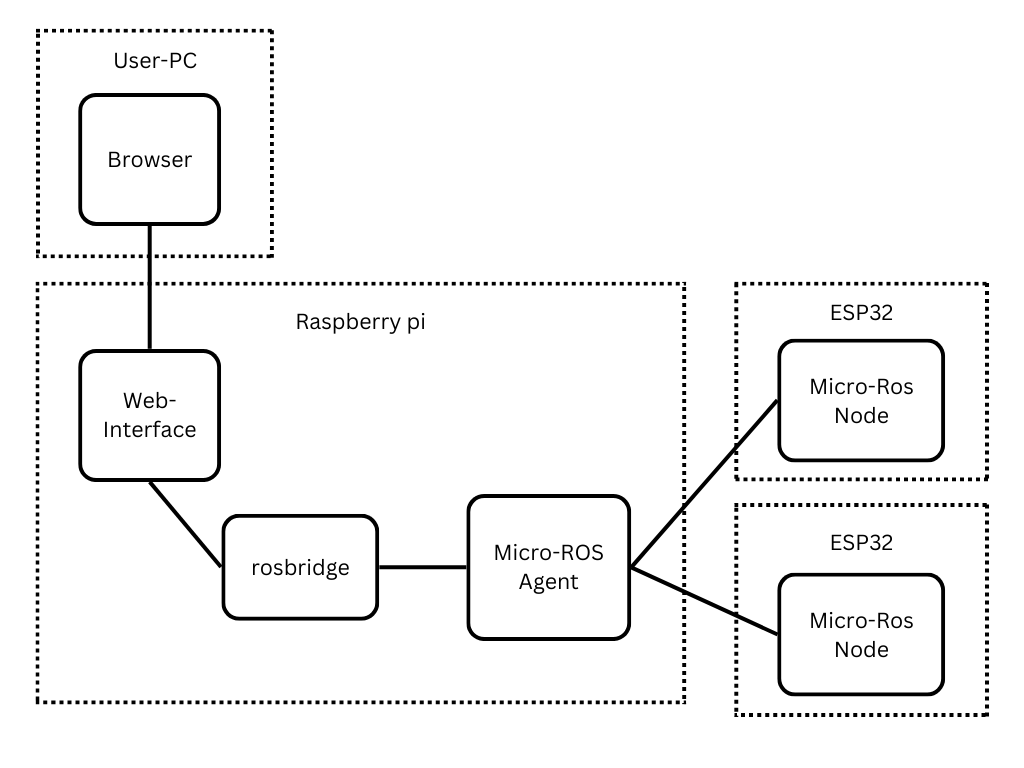
\includegraphics[width=0.8\textwidth]{imgs/Full_system_graph.png}
        \caption{komplette Orchestrierungssoftware}
        \label{fig:orchestration_system}%
    \end{figure}





\end{flushleft}